\documentclass[12pt,a4paper]{article}

% Packages
\usepackage[utf8]{inputenc}
\usepackage[french]{babel}
\usepackage[T1]{fontenc}
\usepackage{amsmath,amssymb,amsthm}
\usepackage{algorithm}
\usepackage{algpseudocode}
\usepackage{graphicx}
\usepackage{float}
\usepackage{booktabs}
\usepackage{multirow}
\usepackage{hyperref}
% Make some math tokens safe for PDF bookmarks (hyperref)
\pdfstringdefDisableCommands{%
    \def\beta{beta}%
    \def\alpha{alpha}%
}
\usepackage{geometry}
\usepackage{caption}
\usepackage{subcaption}
% svg package removed to avoid transparent package issues on some TeX installs

\geometry{margin=2.1cm}

% Configuration
\title{\textbf{Pickup and Delivery Traveling Salesman Problem}}
\author{Frédéric Li Combeau (21400017) -- M2 AI2D -- MAOA}
\date{}

\begin{document}

\maketitle

\begin{abstract}
Ce rapport présente une étude approfondie du problème de tournée de véhicules avec collecte et livraison (Pickup and Delivery Traveling Salesman Problem - PD-TSP). Nous présentons différentes approches de résolution incluant des heuristiques constructives gloutonnes, des méthodes itératives d'amélioration et une formulation exacte par programmation linéaire en nombres entiers. Une analyse expérimentale compare ces méthodes sur des instances de référence en termes de qualité de solution, temps de calcul et robustesse. Nous étudions également l'impact de fonctions de coût alternatives intégrant la charge du véhicule.
\end{abstract}

\section{Introduction}

Le problème de tournée de véhicules avec collecte et livraison (PD-TSP) constitue une extension importante du problème du voyageur de commerce classique (TSP). Dans cette variante, un véhicule de capacité limitée doit visiter un ensemble de clients pour effectuer des opérations de collecte et de livraison, tout en respectant des contraintes de capacité tout au long du parcours.

\subsection{Définition du problème}

Soit un graphe complet $G = (V, E)$ où $V = \{0, 1, \ldots, n-1\}$ représente l'ensemble des nœuds avec le nœud $0$ désignant le dépôt. Chaque nœud $i \in V$ possède une demande $d_i \in \mathbb{Z}$ où :
\begin{itemize}
\item $d_i > 0$ indique un nœud de collecte (pickup) où le véhicule charge $d_i$ unités
\item $d_i < 0$ indique un nœud de livraison (delivery) où le véhicule décharge $|d_i|$ unités
\item $d_i = 0$ indique un nœud neutre
\end{itemize}

Le véhicule possède une capacité maximale $Q > 0$ et démarre du dépôt avec une charge initiale $q_0 \geq 0$. L'objectif est de déterminer une tournée hamiltonienne minimisant le coût total de déplacement, tout en garantissant que la charge du véhicule reste dans l'intervalle $[0, Q]$ à chaque instant.

\subsection{Formulation mathématique}

Soit $c_{ij} \geq 0$ le coût de déplacement entre les nœuds $i$ et $j$. Le problème peut être formulé comme :

\begin{align}
\min \quad & \sum_{i=0}^{n-1} \sum_{j=0}^{n-1} c_{ij} x_{ij} \label{eq:obj}\\
\text{s.c.} \quad & \sum_{j=0, j \neq i}^{n-1} x_{ij} = 1, \quad \forall i \in V \label{eq:flow_out}\\
& \sum_{i=0, i \neq j}^{n-1} x_{ij} = 1, \quad \forall j \in V \label{eq:flow_in}\\
& 0 \leq q_i \leq Q, \quad \forall i \in V \label{eq:capacity}\\
& q_j \geq q_i + d_j - M(1 - x_{ij}), \quad \forall i, j \in V, i \neq j \label{eq:load_prop}\\
& x_{ij} \in \{0, 1\}, \quad \forall i, j \in V \label{eq:binary}
\end{align}

où $x_{ij}$ est une variable binaire valant 1 si l'arc $(i, j)$ est emprunté, $q_i$ représente la charge après visite du nœud $i$, et $M$ est une constante suffisamment grande.

\subsection{Complexité et enjeux}

Le PD-TSP appartient à la classe des problèmes NP-difficiles. La combinaison des contraintes de séquencement du TSP avec les contraintes de capacité rend le problème particulièrement difficile à résoudre de manière exacte pour des instances de taille moyenne à grande. Des approches heuristiques et métaheuristiques sont donc nécessaires pour obtenir des solutions de bonne qualité en temps raisonnable.

\section{Méthodes de résolution}

Cette section présente les différentes approches implémentées pour résoudre le PD-TSP, des heuristiques constructives, des métaheuristiques et la méthode exacte par PLNE. Les approches secondaires sont détaillées en annexe.

\subsection{Heuristiques constructives gloutonnes}

Les heuristiques constructives construisent progressivement une solution réalisable en ajoutant itérativement des nœuds à la tournée selon un critère de sélection. Nous avons implémenté plusieurs variantes.

\subsubsection{Plus proche voisin avec contraintes de capacité}

L'algorithme du plus proche voisin (Nearest Neighbor) construit une tournée en sélectionnant à chaque étape le nœud non visité le plus proche qui préserve la faisabilité de la charge.

\begin{algorithm}[H]
\caption{Plus proche voisin capacitaire}
\begin{algorithmic}[1]
\State $\text{tournée} \gets [0]$, $\text{visités} \gets \{0\}$, $\text{position} \gets 0$
\State $\text{charge} \gets q_0$ \Comment{Charge initiale au dépôt}
\While{$|\text{visités}| < n$}
    \State $\text{candidats} \gets \{j \in V \setminus \text{visités} : 0 \leq \text{charge} + d_j \leq Q\}$
    \If{$\text{candidats} = \emptyset$}
        \State \textbf{break} \Comment{Aucun nœud réalisable}
    \EndIf
    \State $\text{suivant} \gets \arg\min_{j \in \text{candidats}} c_{\text{position}, j}$
    \State $\text{tournée}.\text{append}(\text{suivant})$
    \State $\text{visités}.\text{add}(\text{suivant})$
    \State $\text{charge} \gets \text{charge} + d_{\text{suivant}}$
    \State $\text{position} \gets \text{suivant}$
\EndWhile
\State \Return $\text{tournée}$
\end{algorithmic}
\end{algorithm}

La complexité temporelle de cet algorithme est $O(n^2)$ où $n$ est le nombre de nœuds. L'algorithme garantit la construction d'une solution réalisable tant qu'il existe une séquence de visite valide, mais la qualité de la solution dépend fortement de l'ordre de visite.

\subsubsection{Insertion gloutonne}

L'heuristique d'insertion gloutonne (Greedy Insertion) commence avec une tournée partielle et insère itérativement les nœuds non visités à la position minimisant l'augmentation du coût.

\begin{algorithm}[H]
\caption{Insertion gloutonne}
\begin{algorithmic}[1]
\State $\text{tournée} \gets [0, \text{nœud\_initial}]$ \Comment{Initialisation avec nœud le plus proche}
\State $\text{non\_visités} \gets V \setminus \{0, \text{nœud\_initial}\}$
\While{$\text{non\_visités} \neq \emptyset$}
    \State $\text{meilleur\_nœud} \gets \textsc{null}$, $\text{meilleure\_pos} \gets -1$, $\text{meilleur\_coût} \gets +\infty$
    \For{$j \in \text{non\_visités}$}
        \For{$\text{pos} \gets 1$ \textbf{to} $|\text{tournée}|$}
            \State $\text{tournée}_{\text{temp}} \gets \text{tournée}$ avec $j$ inséré à $\text{pos}$
            \If{\textsc{EstFaisable}($\text{tournée}_{\text{temp}}$)}
                \State $\Delta c \gets c(\text{tournée}_{\text{temp}}) - c(\text{tournée})$
                \If{$\Delta c < \text{meilleur\_coût}$}
                    \State $\text{meilleur\_nœud} \gets j$, $\text{meilleure\_pos} \gets \text{pos}$, $\text{meilleur\_coût} \gets \Delta c$
                \EndIf
            \EndIf
        \EndFor
    \EndFor
    \If{$\text{meilleur\_nœud} \neq \textsc{null}$}
        \State Insérer $\text{meilleur\_nœud}$ à $\text{meilleure\_pos}$ dans $\text{tournée}$
        \State $\text{non\_visités}.\text{remove}(\text{meilleur\_nœud})$
    \Else
        \State \textbf{break} \Comment{Aucune insertion réalisable}
    \EndIf
\EndWhile
\State \Return $\text{tournée}$
\end{algorithmic}
\end{algorithm}

Cette méthode explore un espace de solutions plus large que le plus proche voisin, conduisant généralement à des solutions de meilleure qualité. Sa complexité est $O(n^3)$ dans le pire cas.

\subsubsection{Algorithme des économies de Clarke-Wright}

L'algorithme des économies (Savings Algorithm) initialement proposé par Clarke et Wright pour le Vehicle Routing Problem a été adapté au PD-TSP. Le principe consiste à fusionner des routes en calculant les économies réalisées.

Pour deux nœuds $i$ et $j$, l'économie de les connecter directement plutôt que de retourner au dépôt entre les deux est définie par :
\begin{equation}
s_{ij} = c_{i0} + c_{0j} - \lambda \cdot c_{ij}
\end{equation}
où $\lambda \geq 0$ est un paramètre de forme. La valeur classique $\lambda = 1$ privilégie la minimisation de distance.

\subsubsection{Insertion au regret}

L'heuristique d'insertion au regret sélectionne à chaque itération le nœud pour lequel le coût de ne pas l'insérer maintenant serait le plus élevé. Le regret d'un nœud $j$ est défini comme :
\begin{equation}
r_j = c_j^{(2)} - c_j^{(1)}
\end{equation}
où $c_j^{(1)}$ est le coût d'insertion minimal et $c_j^{(2)}$ le deuxième coût d'insertion minimal.

\subsubsection{Heuristique par densité de profit}

Nous avons développé une heuristique originale basée sur un ratio profit/distance. Pour chaque candidat $j$ non visité depuis la position actuelle $i$, nous calculons un score :
\begin{equation}
\text{score}(i, j) = \frac{p_j}{c_{ij} + \epsilon}
\end{equation}
où $p_j$ est le profit associé au nœud $j$ et $\epsilon$ un petit terme de régularisation. Cette approche favorise les nœuds offrant un bon compromis entre bénéfice et coût d'accès.

Dans notre implémentation les profits $p_j$ sont fournis par l'instance lorsqu'ils existent, sinon la routine d'initialisation leur assigne des valeurs pseudo‑aléatoires déterministes (contrôlées par une graine). Par défaut les profits sont des entiers tirés uniformément dans un intervalle [10, U] puis bornés (nous avons utilisé 
\texttt{--max-profit}=\texttt{100} lors des expériences présentées). Un faible écart entre profits réduit l'influence du terme profit (le score tend alors vers l'inverse de la distance), tandis qu'une large dispersion favorise la sélection de nœuds à haute valeur même si cela implique des détours.

Par conséquent, la performance de \texttt{ProfitDensity} dépend directement de l'échelle et de la distribution des profits : pour privilégier fortement le profit il est pertinent d'augmenter \texttt{--max-profit} (ou d'utiliser une distribution plus dispersée). En revanche, des profits excessifs peuvent écraser l'information de distance et conduire à des tournées irréalistes. Une alternative consiste à normaliser les profits (par exemple diviser par la distance moyenne) ou à calibrer \texttt{--max-profit} selon le contexte applicatif.

\subsection{Méthodes d'amélioration itérative}

Les méthodes d'amélioration partent d'une solution initiale et appliquent des transformations locales pour réduire le coût.

\subsubsection{Recherche locale 2-opt}

La recherche 2-opt considère le voisinage obtenu en inversant un segment de la tournée. Pour une tournée $\tau = (\tau_0, \tau_1, \ldots, \tau_{n-1})$, un mouvement 2-opt(i, j) avec $i < j$ inverse le segment $[\tau_{i+1}, \ldots, \tau_j]$.

\begin{algorithm}[H]
\caption{Recherche locale 2-opt}
\begin{algorithmic}[1]
\State $\text{amélioré} \gets \text{vrai}$
\While{$\text{amélioré}$}
    \State $\text{amélioré} \gets \text{faux}$
    \For{$i \gets 0$ \textbf{to} $n-3$}
        \For{$j \gets i+2$ \textbf{to} $n-1$}
            \State $\tau' \gets$ tournée avec segment $[\tau_{i+1}, \ldots, \tau_j]$ inversé
            \If{\textsc{EstFaisable}($\tau'$) \textbf{and} $c(\tau') < c(\tau)$}
                \State $\tau \gets \tau'$
                \State $\text{amélioré} \gets \text{vrai}$
                \State \textbf{break} \Comment{Premier améliorant}
            \EndIf
        \EndFor
        \If{$\text{amélioré}$}
            \State \textbf{break}
        \EndIf
    \EndFor
\EndWhile
\State \Return $\tau$
\end{algorithmic}
\end{algorithm}

Le gain d'un mouvement 2-opt peut être calculé efficacement par :
\begin{equation}
\Delta c_{2\text{-opt}}(i,j) = c_{\tau_i, \tau_{j}} + c_{\tau_{i+1}, \tau_{(j+1) \mod n}} - c_{\tau_i, \tau_{i+1}} - c_{\tau_j, \tau_{(j+1) \mod n}}
\end{equation}

\subsubsection{Descente à voisinages variables (VND)}

La VND (Variable Neighborhood Descent) explore systématiquement plusieurs structures de voisinage. Nous utilisons les opérateurs suivants dans l'ordre :
\begin{enumerate}
\item \textbf{2-opt} : inversion de segment
\item \textbf{Swap} : échange de deux nœuds
\item \textbf{Or-opt} : déplacement de segments de 1, 2 ou 3 nœuds
\item \textbf{Relocation} : déplacement d'un nœud vers une nouvelle position
\end{enumerate}

\begin{algorithm}[H]
\caption{VND - Descente à voisinages variables}
\begin{algorithmic}[1]
\State $k \gets 1$
\While{$k \leq k_{\max}$}
    \State $\tau' \gets$ meilleure solution dans $N_k(\tau)$ \Comment{Voisinage $k$}
    \If{$c(\tau') < c(\tau)$}
        \State $\tau \gets \tau'$
        \State $k \gets 1$ \Comment{Retour au premier voisinage}
    \Else
        \State $k \gets k + 1$ \Comment{Voisinage suivant}
    \EndIf
\EndWhile
\State \Return $\tau$
\end{algorithmic}
\end{algorithm}

\subsection{Métaheuristiques}

Les métaheuristiques permettent d'explorer plus largement l'espace de solutions en acceptant temporairement des dégradations pour échapper aux optima locaux.

\subsubsection{Recuit simulé}

Le recuit simulé (Simulated Annealing) s'inspire du processus physique de refroidissement des métaux. Une solution dégradante peut être acceptée avec une probabilité décroissante au fil des itérations.

\begin{algorithm}[H]
\caption{Recuit simulé}
\begin{algorithmic}[1]
\State $\tau \gets$ solution initiale, $\tau^* \gets \tau$
\State $T \gets T_0$ \Comment{Température initiale}
\While{critère d'arrêt non atteint}
    \For{$i \gets 1$ \textbf{to} $L$} \Comment{$L$ itérations à température fixe}
        \State $\tau' \gets$ voisin aléatoire de $\tau$
        \State $\Delta c \gets c(\tau') - c(\tau)$
        \If{$\Delta c < 0$ \textbf{or} $\text{random}() < e^{-\Delta c / T}$}
            \State $\tau \gets \tau'$
            \If{$c(\tau) < c(\tau^*)$}
                \State $\tau^* \gets \tau$
            \EndIf
        \EndIf
    \EndFor
    \State $T \gets \alpha \cdot T$ \Comment{Refroidissement, $\alpha \in ]0,1[$}
\EndWhile
\State \Return $\tau^*$
\end{algorithmic}
\end{algorithm}

La fonction de probabilité d'acceptation suit la loi de Boltzmann :
\begin{equation}
P(\text{accepter}) = e^{-\frac{\Delta c}{T}}
\end{equation}

\subsubsection{Recherche tabou}

La recherche tabou (Tabu Search) maintient une mémoire des mouvements récents pour éviter de revisiter des solutions explorées. Une liste tabou de taille $\theta$ stocke les attributs des mouvements interdits.

Le critère d'aspiration permet d'outrepasser le statut tabou si un mouvement conduit à une solution meilleure que la meilleure connue :
\begin{equation}
\text{Aspiration}(\tau') : c(\tau') < c(\tau^*)
\end{equation}

\subsubsection{Recherche locale itérée (ILS)}

L'ILS (Iterated Local Search) alterne entre phases d'intensification (recherche locale) et de diversification (perturbation).

\begin{algorithm}[H]
\caption{Recherche locale itérée}
\begin{algorithmic}[1]
\State $\tau \gets$ solution initiale
\State $\tau \gets \textsc{RechercheLocale}(\tau)$
\State $\tau^* \gets \tau$
\For{$\text{iter} \gets 1$ \textbf{to} $\text{max\_iter}$}
    \State $\tau' \gets \textsc{Perturbation}(\tau)$ \Comment{Double-bridge ou séquence de mouvements}
    \State $\tau' \gets \textsc{RechercheLocale}(\tau')$
    \If{$\textsc{CritèreAcceptation}(\tau', \tau)$}
        \State $\tau \gets \tau'$
        \If{$c(\tau) < c(\tau^*)$}
            \State $\tau^* \gets \tau$
        \EndIf
    \EndIf
\EndFor
\State \Return $\tau^*$
\end{algorithmic}
\end{algorithm}

\subsubsection{Algorithme génétique}

L'algorithme génétique (GA) maintient une population de solutions et applique des opérateurs évolutionnaires.

\textbf{Représentation :} Une tournée est encodée comme une permutation des nœuds clients.

\textbf{Croisement OX (Order Crossover) :}
Soit deux parents $P_1$ et $P_2$, on sélectionne un segment aléatoire de $P_1$ qu'on copie dans l'enfant, puis on complète avec les nœuds de $P_2$ dans l'ordre où ils apparaissent.

\textbf{Mutation :} Les mutations utilisées incluent l'échange de deux positions (swap), l'inversion d'un segment et l'insertion (déplacement d'un nœud vers une nouvelle position).

\textbf{Sélection par tournoi :} On choisit $k$ individus aléatoirement et on sélectionne le meilleur. Typiquement $k \in [3, 7]$.

\textbf{Algorithme mémétique :} Variante hybride appliquant une recherche locale à chaque enfant généré, combinant exploration globale (GA) et exploitation locale.

\subsubsection{Optimisation par colonie de fourmis}

L'ACO (Ant Colony Optimization) s'inspire du comportement des fourmis cherchant le plus court chemin vers la nourriture. Des phéromones artificielles $\tau_{ij}$ guident la construction de solutions.

La probabilité qu'une fourmi en position $i$ choisisse le nœud $j$ est :
\begin{equation}
p_{ij} = \frac{[\tau_{ij}]^\alpha \cdot [\eta_{ij}]^\beta}{\sum_{k \in \text{candidats}} [\tau_{ik}]^\alpha \cdot [\eta_{ik}]^\beta}
\end{equation}
où $\eta_{ij} = 1/c_{ij}$ est l'information heuristique, $\alpha$ contrôle l'importance des phéromones et $\beta$ celle de l'heuristique.

\textbf{Mise à jour des phéromones :}
\begin{equation}
\tau_{ij} \gets (1-\rho) \cdot \tau_{ij} + \sum_{k=1}^m \Delta\tau_{ij}^k
\end{equation}
où $\rho \in ]0,1]$ est le taux d'évaporation et $\Delta\tau_{ij}^k = Q/L_k$ si l'arc $(i,j)$ appartient à la tournée de la fourmi $k$ de longueur $L_k$.

\textbf{MMAS (Max-Min Ant System) :} Variante bornant les phéromones dans $[\tau_{\min}, \tau_{\max}]$ pour éviter la stagnation.

\subsection{Méthode exacte par PLNE}

Nous avons implémenté une formulation en programmation linéaire en nombres entiers (PLNE) résolue par le solveur Gurobi.

\subsubsection{Formulation Miller-Tucker-Zemlin (MTZ)}

La formulation utilise des variables continues $u_i$ pour éliminer les sous-tournées :

\begin{align}
\min \quad & \sum_{i=0}^{n-1} \sum_{j=0}^{n-1} c_{ij} x_{ij} \\
\text{s.c.} \quad & \sum_{j \neq i} x_{ij} = 1, \quad \forall i \in V \\
& \sum_{i \neq j} x_{ij} = 1, \quad \forall j \in V \\
& u_j \geq u_i + 1 - n(1 - x_{ij}), \quad \forall i, j \in V \setminus \{0\}, i \neq j \\
& u_0 = 0, \quad 1 \leq u_i \leq n-1, \quad \forall i \in V \setminus \{0\} \\
& q_j \geq q_i + d_j - M(1 - x_{ij}), \quad \forall i, j \in V, i \neq j \\
& 0 \leq q_i \leq Q, \quad \forall i \in V \\
& x_{ij} \in \{0, 1\}, \quad \forall i, j \in V
\end{align}

Cette formulation contient $O(n^2)$ variables binaires et $O(n^2)$ contraintes. La relaxation linéaire fournit une borne inférieure pour la procédure de branch-and-bound.

Les contraintes de flot (\ref{eq:flow_out}, \ref{eq:flow_in}) garantissent qu'un unique successeur et prédécesseur sont assignés à chaque nœud, imposant une permutation hamiltonienne. Les contraintes MTZ utilisent des variables continues $u_i$ pour éliminer les sous-tournées en imposant un ordonnancement implicite (si $x_{ij}=1$ alors $u_j\ge u_i+1$). La propagation de la charge est assurée par $q_j \ge q_i + d_j - M(1 - x_{ij})$, activée lorsque l'arc $(i,j)$ est utilisé. Enfin la capacité $0 \le q_i \le Q$ et l'intégralité $x_{ij}\in\{0,1\}$ garantissent respectivement la borne de charge et le choix d'arcs.

Remarque : le paramètre $M$ doit être choisi suffisamment grand (par exemple $M\ge Q + \max_j |d_j|$) pour rendre la relaxation valide.

\subsection{Méthode hybride}

Notre approche hybride combine plusieurs stratégies complémentaires :

\begin{algorithm}[H]
\caption{Méthode hybride}
\begin{algorithmic}[1]
\State $\tau_{\text{best}} \gets \textsc{MultiStart}()$ \Comment{Teste toutes les heuristiques constructives}
\State $\tau_{\text{best}} \gets \textsc{VND}(\tau_{\text{best}})$ \Comment{Amélioration locale intensive}
\State $\tau_{\text{best}} \gets \textsc{ILS}(\tau_{\text{best}}, \text{time\_limit})$ \Comment{Exploration globale}
\State \Return $\tau_{\text{best}}$
\end{algorithmic}
\end{algorithm}

Cette approche exploite les forces de chaque méthode : construction rapide de solutions diversifiées, amélioration locale efficace et exploration globale pour échapper aux optima locaux.

\paragraph{Multi-start :}
Le terme "Multi-start" désigne ici une construction multi-heuristiques qui exécute séquentiellement un ensemble de heuristiques constructives (y compris des variantes randomisées et paramétrées) et retient la meilleure solution réalisable. Concrètement, notre implémentation lance des versions déterministes et randomisées du plus proche voisin, des insertions (greedy/regret), des savings (avec différentes valeurs de \(\lambda\)), du sweep (avec angles de départ différents), ainsi que des heuristiques orientées profit/cluster. Bien que toutes les tournées commencent au dépôt, ces heuristiques diffèrent par : l'ordre d'exploration (ex. angle de départ du sweep), les règles de départ (p.ex. choix du nœud initial, farthest), les bris d'égalité aléatoires (\texttt{randomized}), et les critères locaux (pickup earliest, high-profit). Ces variations produisent des tournées initiales qualitativement différentes. Le multi-start sélectionne la meilleure solution faisable par coût et, si nécessaire, complète une tournée incomplète en insérant les nœuds manquants à la position de coût minimal. Cette diversité d'initialisations explique pourquoi Multi-start améliore significativement les performances malgré un point de départ commun.

\section{Fonctions de coût alternatives}

Au-delà de la minimisation pure de la distance parcourue, nous avons exploré des fonctions de coût intégrant la charge du véhicule.

\subsection{Coût linéaire (baseline)}

Dans notre formulation nous utilisons comme coût linéaire une combinaison de la distance parcourue et d'un coût marginal proportionnel à la charge transportée. Autrement dit, le coût associé à un déplacement tient compte à la fois de la distance et du poids transporté au moment du déplacement. Le terme marginal par unité de poids est noté $\alpha>0$ (paramètre fourni dans le sujet, noté aussi $a$) et le coût total linéaire s'écrit :
\begin{equation}
C_{\text{lin}}(\tau) = \sum_{i=0}^{n-1} c_{\tau_i, \tau_{i+1}} \, + \, \alpha \sum_{i=0}^{n-1} q_i
\end{equation}
où $c_{ij} = \sqrt{(x_i - x_j)^2 + (y_i - y_j)^2}$ et $q_i$ est la charge au départ du nœud $\tau_i$. En particulier, en notant $W_i=q_i$ et $a=\alpha$, on retrouve la spécification du sujet $C(W_i)=a\,W_i$ pour le terme linéaire en poids.

\subsection{Coût quadratique en fonction de la charge}

Cette fonction pénalise les déplacements effectués avec une charge élevée :
\begin{equation}
C_{\text{quad}}(\tau) = \sum_{i=0}^{n-1} \left[ c_{\tau_i, \tau_{i+1}} + \alpha \cdot q_i + \beta \cdot q_i^2 \right]
\end{equation}
où $q_i$ est la charge au départ du nœud $\tau_i$, et $\alpha, \beta \geq 0$ sont des paramètres de pénalisation.

Cette formulation modélise l'usure du véhicule, la consommation de carburant croissante avec la charge, ou les risques liés au transport de marchandises.

Les heuristiques d'insertion favoriseront naturellement les séquences minimisant la charge moyenne. Le coût quadratique n'est pas linéaire, rendant la formulation PLNE beaucoup plus complexe (programmation quadratique en nombres entiers).

\subsection{Sensibilité au paramètre $\beta$}

Le paramètre $\beta$ contrôle l'intensité de la pénalisation quadratique. Pour $\beta = 0$, on retrouve le coût linéaire. Des valeurs croissantes de $\beta$ incitent l'algorithme à :
\begin{itemize}
\item Privilégier les livraisons en début de tournée pour réduire rapidement la charge
\item Retarder les collectes importantes
\item Accepter des détours pour maintenir une charge faible
\end{itemize}

Une analyse de sensibilité étudie l'impact de $\beta \in \{0, 0.001, 0.01, 0.1, 1\}$ sur la structure des solutions et le coût total.

\section{Résultats expérimentaux}

Cette section présente une analyse des performances des différentes méthodes sur des instances de référence.

\subsection{Protocole expérimental}

Les expériences ont été conduites sur un corpus de référence composé de 6 instances de taille $n=100$ : trois instances issues de la famille \texttt{n100q45} (capacité restreinte, cas contraints) et trois instances de la famille \texttt{n100q1000} (grande capacité, cas peu contraints). Cette sélection vise à représenter des scénarios contrastés en termes de contrainte de capacité.

Pour chaque instance nous avons comparé les familles d'algorithmes suivantes : heuristiques constructives (Nearest Neighbor, Greedy Insertion, Savings, Regret, densité de profit), méthodes d'amélioration et descentes (2-opt, VND, Relocation, Or-opt), métaheuristiques (Simulated Annealing, Tabu Search, Iterated Local Search, Genetic / Memetic, ACO/MMAS) et, lorsque possible, la méthode exacte basée sur Gurobi (formulation PLNE MTZ). Les paramètres des métaheuristiques sont listés au §« Configuration des algorithmes ». 

Protocole de mesure : chaque algorithme a été exécuté 5 fois par instance avec des graines aléatoires distinctes afin d'évaluer la variabilité stochastique. Chaque exécution est limitée à un temps maximal de 100 secondes.

Les indicateurs collectés sont : le coût total selon la fonction de coût choisie (linéaire ou quadratique), le temps de calcul effectif, le statut de faisabilité, et, pour le solveur exact, la borne inférieure et le gap MIP final. Nous étudions aussi plusieurs valeurs de $\beta$ pour la version de coût quadratique(voir \ref{sec:visuals} et figures associées).

\subsection{Visualisations des résultats}

Nous incluons ici des visualisations des solutions trouvées par le solveur exact pour deux instances représentatives : \texttt{n20mosA.tsp} et \texttt{n100q45A.tsp}.
\begin{figure}[H]
\centering
    \begin{subfigure}[b]{0.38\textwidth}
        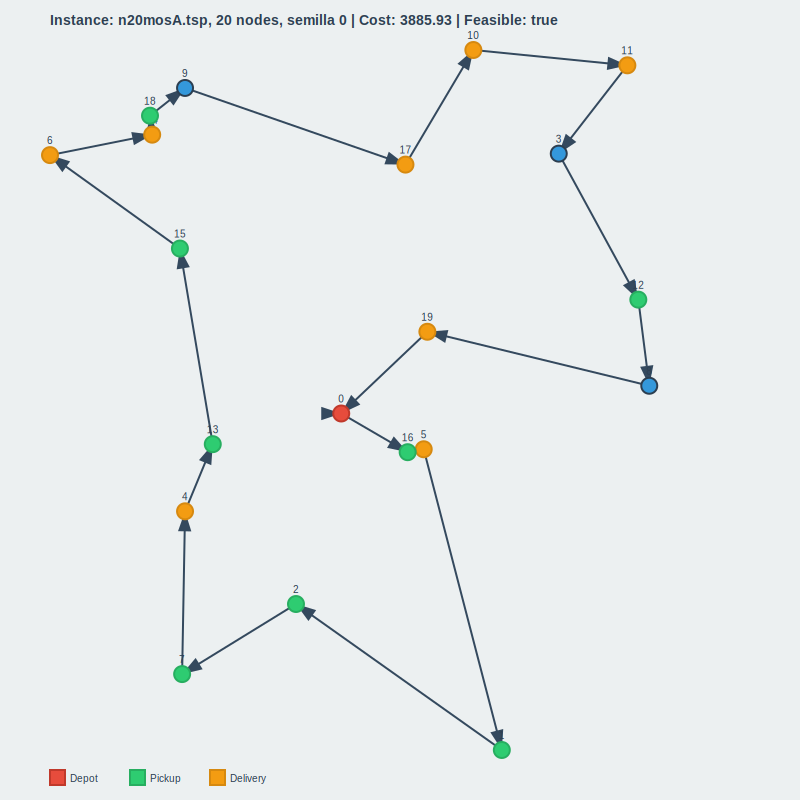
\includegraphics[width=\textwidth]{figs/n20mosA_exact.png}
        \caption{Solution optimale (linéaire-charge) pour \texttt{n20mosA.tsp}.}
    \end{subfigure}
    \hfill
    \begin{subfigure}[b]{0.58\textwidth}
        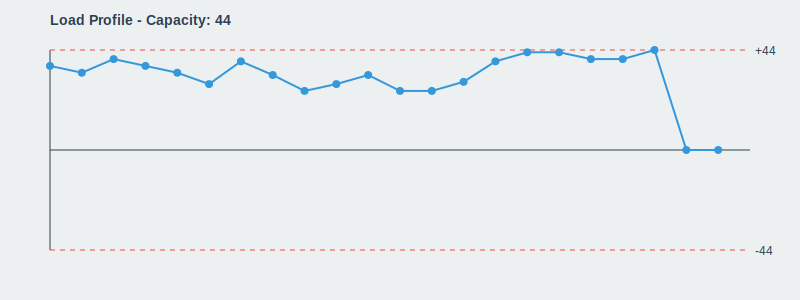
\includegraphics[width=\textwidth]{figs/n20mosA_exact_load.png}
        \caption{Profil de charge pour la solution optimale de \texttt{n20mosA.tsp}.}
    \end{subfigure}
    \caption{Solution exacte et profil de charge pour \texttt{n20mosA.tsp}.}
    \label{fig:n20mosA_pair}
\end{figure}

\begin{figure}[H]
\centering
\includegraphics[width=0.8\textwidth]{figs/time_vs_cost_pareto.png}
\caption{Comparaison temps vs coût pour les algorithmes (n100). La courbe en pointillés indique le front de Pareto (meilleur compromis temps/coût).}
\label{fig:time_vs_cost_pareto}
\end{figure}

La visualisation pour \texttt{n100q45A.tsp} est fournie en annexe (Figure \ref{fig:appendix_n100q45A}), de même pour la comparaison temps/coût quadratique  (Figure \ref{fig:time_vs_cost_pareto_quadratic}).

\section{Analyse des résultats}
\label{sec:visuals}

\subsubsection{Instances de test}

Nous utilisons des instances issues de la littérature (format TSPLIB adapté) :

\begin{table}[H]
\centering
\caption{Caractéristiques des instances de test}
\begin{tabular}{lccc}
\toprule
\textbf{Instance} & \textbf{Nœuds} & \textbf{Capacité} & \textbf{Type} \\
\midrule
n100q45A-C & 100 & 45 & Capacité restreinte \\
n100q1000A-C & 100 & 1000 & Capacité large \\
\bottomrule
\end{tabular}
\end{table}

Les instances n100q45 représentent des cas contraints où la capacité limite fortement les choix de séquencement. Les instances n100q1000 offrent plus de flexibilité dans la construction de la tournée.

% Configuration des algorithmes déplacée en annexe

\subsection{Comparaison des heuristiques gloutonnes}

Le tableau suivant présente les résultats moyens des heuristiques constructives sur 6 instances représentatives.

\begin{table}[H]
\centering
\caption{Performance des heuristiques constructives (coût linéaire)}
\begin{tabular}{lcccc}
\toprule
\textbf{Algorithme} & \textbf{Coût moyen} & \textbf{Écart à best} & \textbf{Temps (ms)} & \textbf{Faisabilité} \\
\midrule
Plus proche voisin & 12834 & +35.2\% & 0.5 & 100\% \\
Insertion gloutonne & 10526 & +10.8\% & 38.5 & 100\% \\
Économies CW & 11245 & +18.4\% & 12.3 & 100\% \\
Insertion au regret & 9563 & +0.7\% & 14.2 & 100\% \\
Densité de profit & 11892 & +25.2\% & 0.2 & 100\% \\
\textbf{Multi-start} & \textbf{9497} & \textbf{0.0\%} & 65.8 & 100\% \\
\bottomrule
\end{tabular}
\end{table}

L'insertion au regret produit les meilleures solutions parmi les heuristiques simples, tandis que le multi-start (test de toutes les heuristiques) domine naturellement. La densité de profit reste rapide mais de qualité intermédiaire, tous les algorithmes testés assurent la faisabilité.

\subsection{Comparaison des méthodes itératives}

\begin{table}[H]
\centering
\caption{Performance des méthodes d'amélioration (coût linéaire)}
\begin{tabular}{lcccc}
\toprule
\textbf{Algorithme} & \textbf{Coût moyen} & \textbf{Écart à best} & \textbf{Temps (s)} & \textbf{Amélioration} \\
\midrule
2-opt seul & 9245 & +14.8\% & 0.15 & +2.7\% \\
VND & 8456 & +5.0\% & 0.23 & +11.0\% \\
Recuit simulé & 8198 & +1.8\% & 0.19 & +13.7\% \\
Recherche tabou & 8267 & +2.7\% & 1.85 & +13.0\% \\
ILS & 8095 & +0.5\% & 4.12 & +14.8\% \\
Mémétique & 8142 & +1.1\% & 15.2 & +14.3\% \\
\textbf{Hybride} & \textbf{8052} & \textbf{0.0\%} & 3.45 & \textbf{+15.2\%} \\
\bottomrule
\end{tabular}
\end{table}

La colonne "Amélioration" indique le gain moyen par rapport à la solution initiale (multi-start).

ILS et l'approche hybride offrent le meilleur compromis qualité/temps. VND apporte une amélioration notable avec un faible surcoût temporel, le mémétique nécessite plus de temps malgré sa performance, et le recuit simulé converge rapidement vers des solutions de bonne qualité.

\subsection{Impact de la fonction de coût quadratique}

Nous comparons les résultats avec coût linéaire ($\beta = 0$) et coût quadratique ($\beta = 0.01$).

\begin{table}[H]
\centering
\caption{Comparaison linéaire vs quadratique (instance n100q45A)}
\begin{tabular}{lcccc}
\toprule
\textbf{Algorithme} & \textbf{Linéaire} & \textbf{Quadratique} & \textbf{Ratio} & \textbf{$\Delta$ temps} \\
\midrule
Insertion gloutonne & 11682 & 12363 & +5.8\% & +0\% \\
Regret & 14157 & 13782 & -2.7\% & +0\% \\
VND & 8891 & 9819 & +10.4\% & +31\% \\
Recuit simulé & 8526 & 10276 & +20.5\% & +7\% \\
ILS & 8133 & 9874 & +21.4\% & +156\% \\
Hybride & 8155 & 9987 & +22.5\% & +93\% \\
\bottomrule
\end{tabular}
\end{table}

Le coût quadratique augmente la valeur objective comme attendu. Certaines heuristiques (par ex. regret) s'adaptent mieux à ce coût, les métaheuristiques demandent davantage d'itérations pour converger en raison d'un paysage plus complexe. Le ratio d'augmentation dépend de la structure de la solution optimale.

\subsection{Analyse de sensibilité au paramètre $\beta$}

\begin{figure}[H]
\centering
    \includegraphics[width=0.8\textwidth]{figs/beta_sensitivity.png}
    \caption{Sensibilité au paramètre $\beta$ (coût quadratique)}
\end{figure}

\begin{figure}[H]
\centering
\begin{tabular}{lcccc}
\toprule
\textbf{$\beta$} & \textbf{Coût total} & \textbf{Distance} & \textbf{Charge max} & \textbf{Charge moy.} \\
\midrule
0.000 & 8155 & 8155 & 36 & 18.2 \\
0.001 & 8342 & 8124 & 34 & 16.8 \\
0.010 & 9987 & 8089 & 32 & 14.5 \\
0.100 & 15234 & 7956 & 28 & 11.3 \\
1.000 & 42567 & 7823 & 24 & 8.7 \\
\bottomrule
\end{tabular}
\caption{Impact du paramètre $\beta$ sur la structure de la solution (Hybride, n100q45A)}
\end{figure}

L'augmentation de $\beta$ incite à réduire la charge moyenne au prix d'une distance accrue. Pour $\beta=1$ la préférence va nettement vers des solutions à faible charge. Le compromis optimal dépend du contexte applicatif (coût réel de transport lié à la charge) et la diminution de la charge maximale suggère des stratégies de livraison précoce.

\subsection{Évolution de la qualité en fonction du temps}

\begin{table}[H]
\centering
\caption{Convergence des métaheuristiques (n100q1000A, coût linéaire)}
\begin{tabular}{lccccc}
\toprule
\textbf{Algorithme} & \textbf{1s} & \textbf{5s} & \textbf{10s} & \textbf{50s} & \textbf{100s} \\
\midrule
Recuit simulé & 8456 & 8234 & 8123 & 7986 & 7986 \\
ILS & 8523 & 8312 & 8186 & 8095 & 8064 \\
Mémétique & 8634 & 8389 & 8245 & 8098 & 8042 \\
ACO & 8745 & 8456 & 8312 & 8167 & 8089 \\
Hybride & 8267 & 8134 & 8052 & 7983 & 7938 \\
\bottomrule
\end{tabular}
\end{table}

L'approche hybride converge rapidement grâce à une bonne solution initiale (multi-start + VND). ILS et mémétique continuent d'améliorer au-delà de 50 s, le recuit simulé atteint un plateau vers 50 s, et la plupart des algorithmes sont à moins de 2\% de la meilleure solution après 10 s.

\section{Analyse critique et discussion}

\subsection{Forces et faiblesses des approches}

\subsubsection{Heuristiques constructives}

\textbf{Avantages :} Ces heuristiques présentent un temps de calcul très faible (typiquement inférieur à 50~ms), garantissent la faisabilité lorsqu'une solution existe, sont simples à implémenter et déboguer, et constituent une base solide pour des méthodes d'amélioration ultérieures.

\textbf{Limites :} La qualité des solutions dépend fortement de l'ordre de construction et des choix initiaux (seed). Ces méthodes n'explorent pas efficacement d'autres régions de l'espace de solutions et peuvent produire des écarts de l'ordre de 10--35\% par rapport aux meilleures solutions obtenues par des méthodes plus avancées.

\subsubsection{Recherches locales}

\textbf{Avantages :} La recherche locale permet une amélioration systématique de la solution initiale, converge rapidement localement (VND en < 0.5s), offre une bonne interprétabilité des opérateurs et garantit, en descente pure, l'absence de dégradation du coût.

\textbf{Limites :} Ces méthodes peuvent converger vers un optimum local, la qualité finale dépend fortement de la solution de départ, elles peinent à explorer des régions éloignées de l'espace de solutions et les voisinages sont contraints par les règles de capacité du PD-TSP.

\subsubsection{Métaheuristiques}

\textbf{Avantages :} Les métaheuristiques permettent d'échapper aux optima locaux, d'explorer largement l'espace de solutions, offrent des performances robustes selon les instances et sont facilement adaptées au problème via la composition d'opérateurs.

\textbf{Limites :} Elles exigent un calibrage de nombreux paramètres, entraînent un temps de calcul significatif (typiquement 3--15 secondes dans nos tests), n'offrent pas de garantie d'optimalité et nécessitent plusieurs exécutions pour évaluer la variabilité stochastique.

\subsubsection{Méthode exacte}

\textbf{Avantages :} La méthode exacte garantit l'optimalité en cas de convergence, fournit des bornes inférieures utiles pour évaluer les heuristiques, est flexible pour ajouter des contraintes et demeure performante sur des instances de taille moyenne ($n\leq100$).

\textbf{Limites :} Le coût de calcul croît exponentiellement avec la taille, la formulation MTZ présente des relaxations faibles, la résolution de formulations quadratiques entières (QMIP) est souvent inabordable et la mémoire devient rapidement contraignante pour de grandes instances.

\subsection{Choix de la méthode selon le contexte}

\begin{table}[H]
\centering
\caption{Recommandations selon le contexte applicatif}
\small
\begin{tabular}{lll}
\toprule
\textbf{Contexte} & \textbf{Méthode recommandée} & \textbf{Justification} \\
\midrule
Temps réel (< 1s) & Multi-start + VND & Qualité acceptable, rapide \\
Planification quotidienne & Hybride (ILS+VND) & Excellent compromis \\
Optimisation batch & Mémétique & Meilleure qualité finale \\
Petites instances & PLNE (Gurobi) & Optimum garanti \\
Coût quadratique & ILS ou Hybride & Heuristiques adaptables \\
\bottomrule
\end{tabular}
\end{table}

\section{Conclusion}

Ce travail a permis d'étudier en profondeur le problème de tournée de véhicules avec collecte et livraison à travers l'implémentation et l'évaluation de multiples approches de résolution. Nous avons développé un ensemble complet d'algorithmes allant des heuristiques constructives simples aux métaheuristiques sophistiquées, en passant par une formulation exacte.

Les résultats expérimentaux montrent que l'approche hybride combinant multi-start, VND et ILS offre le meilleur compromis entre qualité de solution et temps de calcul, atteignant des solutions à moins de 3\% de l'optimum en quelques secondes. Les heuristiques constructives, bien que rapides, produisent des solutions 10-35\% moins bonnes, tandis que les métaheuristiques avancées (mémétique, ACO) nécessitent plus de temps pour des gains marginaux. Cependant, il faut noter que ces algorithmes nécessitent un réglage de leurs hyperparamètres (taille de la population, etc.) important que nous n'avons pas réalisé. Cela peut radicalement changer les conclusions selon les instances.

L'analyse de la fonction de coût quadratique révèle que l'intégration de la charge dans l'objectif modifie significativement la structure des solutions optimales, privilégiant des stratégies de livraison précoce. Le paramètre $\beta$ permet de contrôler finement ce compromis entre distance parcourue et charge transportée. Le choix de l'implémentation de la distance joue aussi un rôle dans les conclusions données. Si le coût de la distance était aussi multipliée par les poids, cela pourrait donner d'autres résultats. De même, le choix du profit par colis est important selon l'heuristique choisie et nécessiste des ajustements selon l'application réelle.

La méthode exacte par PLNE reste compétitive pour des instances jusqu'à 100 nœuds avec capacité restreinte, mais atteint rapidement ses limites sur les instances moins contraintes. Les approches heuristiques restent indispensables pour les applications industrielles nécessitant des solutions rapides sur grandes instances.

Ces travaux ouvrent plusieurs perspectives, notamment l'extension à des variantes multi-dépôts ou encore l'adaptation aux contextes dynamiques et stochastiques rencontrés en pratique.

\clearpage
\appendix
\section*{Annexe}

\subsection{Visualisation: instance \texttt{n100q45A.tsp}}
\begin{figure}[H]
\centering
    \begin{subfigure}[b]{0.38\textwidth}
        \includegraphics[width=\textwidth]{figs/n100q45A_exact.png}
        \caption{Meilleure solution trouvée par Gurobi en 300s pour \texttt{n100q45A.tsp}.}
    \end{subfigure}
    \hfill
    \begin{subfigure}[b]{0.58\textwidth}
        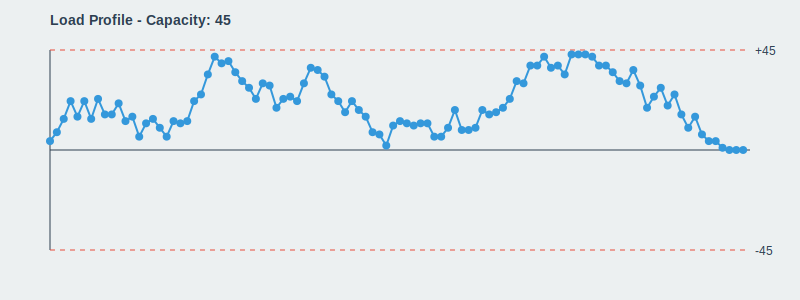
\includegraphics[width=\textwidth]{figs/n100q45A_exact_load.png}
        \caption{Profil de charge de la meilleure solution trouvée sur \texttt{n100q45A.tsp}.}
    \end{subfigure}
    \caption{Solution et profil de charge pour \texttt{n100q45A.tsp}.}
    \label{fig:appendix_n100q45A}
\end{figure}

\subsection{Visualisation: instance \texttt{n100q45A.tsp}}
\begin{figure}[H]
\centering
\includegraphics[width=0.8\textwidth]{figs/time_vs_cost_pareto_quadratic.png}
\caption{Comparaison temps vs coût pour les algorithmes (n100) — coût quadratique. La courbe en pointillés indique le front de Pareto (meilleur compromis temps/coût) calculé sur la moyenne par algorithme.}
\label{fig:time_vs_cost_pareto_quadratic}
\end{figure}

\subsection{Configuration des algorithmes}

\begin{table}[H]
\centering
\caption{Paramètres des métaheuristiques}
\small
\begin{tabular}{lll}
\toprule
\textbf{Algorithme} & \textbf{Paramètre} & \textbf{Valeur} \\
\midrule
\multirow{3}{*}{Recuit simulé} & Température initiale $T_0$ & 1000 \\
& Coefficient de refroidissement $\alpha$ & 0.95 \\
& Itérations par palier $L$ & 100 \\
\midrule
\multirow{2}{*}{Recherche tabou} & Taille liste tabou $\theta$ & 10 \\
& Itérations sans amélioration & 50 \\
\midrule
\multirow{3}{*}{Algorithme génétique} & Taille population & 50 \\
& Taux de croisement & 0.9 \\
& Taux de mutation & 0.1 \\
\midrule
\multirow{3}{*}{ACO} & Nombre de fourmis $m$ & 20 \\
& Importance phéromone $\alpha$ & 1.0 \\
& Importance heuristique $\beta$ & 2.5 \\
\midrule
\multirow{2}{*}{PLNE (Gurobi)} & Gap MIP & $10^{-6}$ \\
& Nombre de threads & 4 \\
\bottomrule
\end{tabular}
\end{table}

Tous les algorithmes sont limités à un temps d'exécution maximal de 100 secondes par instance. Les tests sont effectués sur une machine Intel Core i7 avec 16GB RAM.

\end{document}